\documentclass[../skript.tex]{subfiles}

	\subsection{Directed Hamiltonian Cycle Problem}
		\underline{Input: } A digraph $G$\par
		\underline{Question: } Does $G$ contain a cycle of length $|V(G)|$?

		\begin{theorem}[Karp (Reductability among comb. problems)]\label{thm5}
			Directed Hamiltonian Cycle is NP-complete.
		\end{theorem}
		\begin{proof}
			\begin{figure}\label{fig1}[ht]
				\centering
				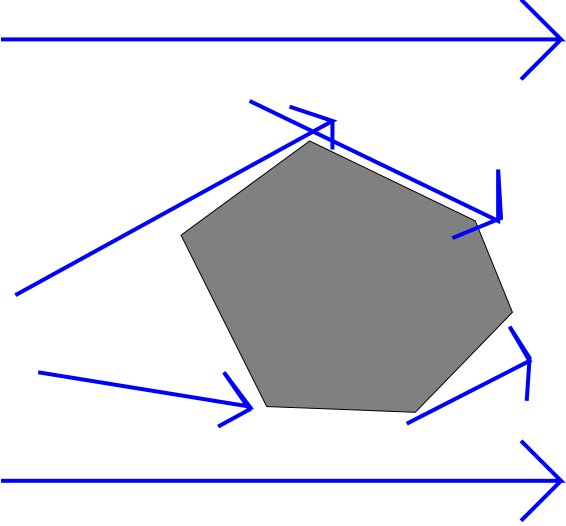
\includegraphics[width=0.5\textwidth]{Images/karp1.png}
				\caption{The path used for the proof of \cref{thm5}}
			\end{figure}
			The problem is obviously in NP. Reduce 3-SAT to Directed Hamiltonian Cycles as follows:\par
			Let $F = C_1\land C_2\land ...\land C_k$ be a 3-SAT formula in variables $x_1,...,x_n$. Construct $G$ as follows: Path $P_i$ for $i=1,...,n$ on $3R+3$ vertices (see \cref{fig1}).
			\begin{figure}\label{fig1}[ht]
				\centering
				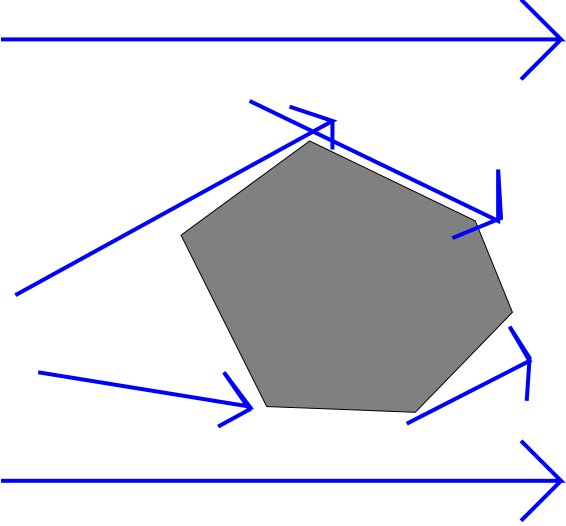
\includegraphics[width=0.5\textwidth]{Images/karp1.png}
				\caption{The path used for the proof of \cref{thm5}}
			\end{figure}
			Add vertices $s$ and $t$ and connect the paths as in \cref{fig2}. For each clause $C_j$ add a vertex $c_j$. Connect $c_j$ with vertex $3j+1$ in $P_i$ and connect vertex $3j$ in $P_i$ with $c_j$ if $x_i$ appears in $C_j$. For $\bar{x}_i$: Reverse direction. $F$ satisfies: Fix some satisfying truth assignment. Traverse $P_i$ rom left to right $\Leftrightarrow$ $x_i$ is true.
			\begin{figure}\label{fig1}[ht]
				\centering
				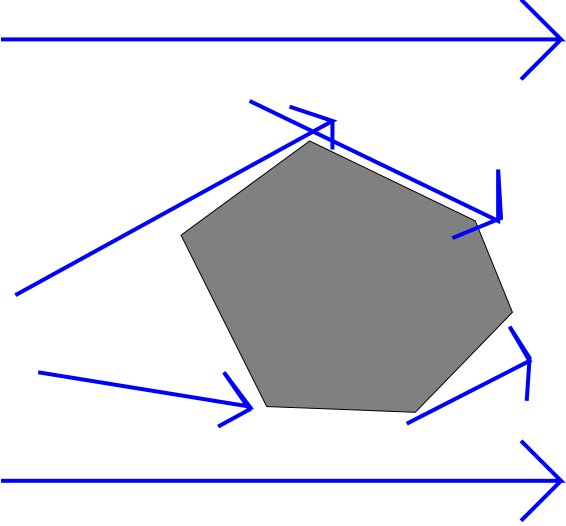
\includegraphics[width=0.5\textwidth]{Images/karp1.png}
				\caption{The path used for the proof of \cref{thm5}}
			\end{figure}
			 Choose for each $C_j$ a true literal (see \cref{fig3}).\par
			 \textbf{Assume:} A directed Hamiltonian Circuit exists. \par
			 \begin{figure}\label{fig1}[ht]
				\centering
				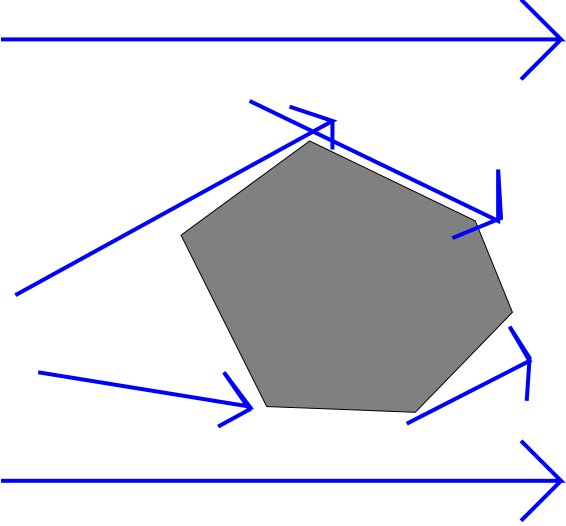
\includegraphics[width=0.5\textwidth]{Images/karp1.png}
				\caption{The path used for the proof of \cref{thm5}}
			\end{figure}
			 \textbf{Observation: } If the circuit enters a vertex $c_j$ from path $P_i$ then the next edge will go back to $P_i$ (see \cref{fig4})
			 $\Rightarrow$ We can remove all the $c_j$ vertices from the hamiltonian circuit by replacing the two edges by one edge from some $P_i$ $\Rightarrow$ Use direction of the $P_i$s as truth values.
		\end{proof}
		\begin{remark}
			The same statement holds for Hamiltonian paths.
		\end{remark}

	\subsection{Vertex Cover}
		\textbf{Input:} A Graph $G=(V,E), R\in\mathbb{N}$\par
		\textbf{Question:} Does $G$ contain an $S\subseteq V$ s.t. $|S|\leq R$ s.t. each edge in $E$ has at least one endpoint in $S$?
		\begin{theorem}[Karp 1972]\label{thm7}
			The Problem of Vertex Cover is NP-Complete.
		\end{theorem}
		\begin{proof}
			Obviously the problem is in NP. Reduce 3-SAT to Vertex Cover. \par
			Let $F=C_1\land...\land C_q$ be a 3-SAT formula. W.l.o.g. each clause contains \underline{exactly} 3 literals. Construct $G$ as follows: $3q$ vertices\par
			Edges: 
			\begin{itemize}
				\item [1)] Connect the three vertices corresponding to the 3 literals of the same clause.
				\item [2)] Connect the vertices $a,b$ if they correspond to negations of each other.
			\end{itemize}
			\begin{figure}\label{fig1}[ht]
				\centering
				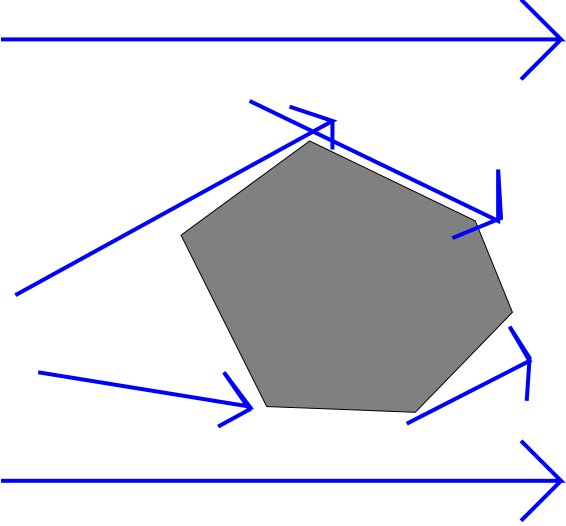
\includegraphics[width=0.5\textwidth]{Images/karp1.png}
				\caption{The constructed Graph for the proof of \cref{thm7}}
			\end{figure}
			\underline{Claim:} $G$ has a vertex cover of size $2q\,\Leftrightarrow$ $F$ is satisfiable.\par
			$F$ is satisfiable $\rightarrow$ Fix some truth assignment. Choose some true literal from each clause. Take all non-chosen vertices as vertex cover. This is really a vertex cover, because we cannot have that $x_i$ and $\bar x_i$ are true for some $i$.\newline\noindent
			$G$ has a vertex cover of size $2q\,\Rightarrow$ vertex cover contains exactly 2 vertices from each triangle (clause). Set all uncovered vertices to true; it is well defined as $\{x_i,\bar x_i\}$ is an edge for all $i$ and ust be covered.
		\end{proof}

	\subsection*{title}{Stable Set}
		\textbf{Input: } A graph $G = (V,E), R\in\mathbb{N}$\par
		\textbf{Question: } Is there an $S\subseteq V$ with $|S|=R$ s.t. no edge in $E$ connects two vertices in $S$?
		\begin{theorem}[Karp]\label{thm8}
			Stable Set is NP-Complete.
		\end{theorem} 
		\begin{proof}
			\underline{Observation:} $S\subseteq V$ is a stable set $\Leftrightarrow$ $V\setminus S$ is a vertex cover. Moreover $S\subseteq V$ is a stable set of size $n-k$ $\Leftrightarrow$ $V\setminus S$ is a vertex cover of size $k$.\par
		\end{proof}
	\subsection*{title}{Clique Problem}
		\textbf{Input: } A graph $G=(V,E), R\in\mathbb{N}$\par
		\textbf{Question: } Is there an $S\subseteq V, |S|=R$ s.t. all possible edges between vertices in $S$ belong to $E$.
		\begin{theorem}[Karp 1972]\label{thm9}
			The Clique Problem is NP-Complete.
		\end{theorem}
		\begin{proof}
			It is obviously in NP. Moreover, $S$ is a stable set in $G$ $\Leftrightarrow$ $S$ is a clique in $\bar{G}$.
		\end{proof}

	\subsection*{title}{Set Cover}
		\textbf{Input:} A family $S_1,...,S_m$ of subsets of a finite set $S$, $R\in\mathbb{N}$\par
		\textbf{Question: } Is there a subfamily $S_{i_1},...,S_{i_R}$ s.t. $\bigcup_{j=1}^R S_{i_j} = S$?
		\begin{theorem}[Karp 1972]\label{thm10}
			Set cover is NP-Complete.
		\end{theorem}
		\begin{proof}
			It is obviously in NP. Reduce Vertex-Cover to Set Cover as follows:\par
			Let $G=(V,E), k\in\mathbb{N}$ be a vertex cover instance. Set $S\coloneqq E$ and $S_x\coloneqq \delta(x)$ for $x\in V(G)$. 
		\end{proof}
	\subsection{Integer Linear Inequalities}
		\textbf{Input: } A matrix $A\in\mathbb{Z}^{m\times n}, b\in\mathbb{Z}^m$\par
		\textbf{Question: } Is there a vector $x\in\mathbb{Z}^n$ s.t. $Ax=b$?
		\begin{theorem}[Karp 1972]\label{thm11}
			Integer Linear Inequalities is NP-Complete
		\end{theorem}
		\begin{proof}
			The problem is in NP. Reduce 3-SAT to Integer Linear Inequalities:\par
			Let $F=C_1\land ...\land C_q$, in the variables $x_1,...,x_n$. We use the following inequalities:
			\begin{equation*}\left.\begin{aligned}
				-x_i-\bar x_i &\leq& -1\\
				x_i+\bar x_i &\leq& 1\\
				-x_i &\leq& 0\\
				-\bar x_i &\leq& 0
				\end{aligned}\right\}\Rightarrow \begin{aligned}
					&x_i - 0 \land \bar x_i = 1\\
					\text{or }\, &x_i = 1 \land \bar x_i = 0
				\end{aligned}
			\end{equation*}
		\end{proof}

	\subsection{3-Dimensional Matching (3DM)}
		\textbf{Input: } Disjoint sets $X,Y,Z$ each of size $n$ and $T\subseteq X\times Y\times Z$ a set of hyperedges\par
		\textbf{Question: } Is there an $M\subset T$ with $|M| = n$ s.t. $\forall x\in X\times Y\times Z$ there exists exactly one $m\in M$ containing $a$?
		\begin{theorem}[Karp 1972]\label{thm12}
			3DM is NP-Complete.
		\end{theorem}
		\begin{proof}
			Obviously 3DM is in NP. Reduce 3-SAT to 3DM as follows:\par
			\begin{figure}\label{fig6}[ht]
				\centering
				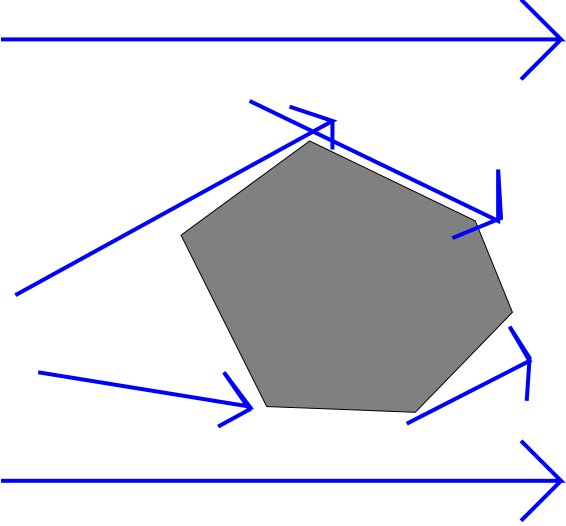
\includegraphics[width=0.5\textwidth]{Images/karp1.png}
				\caption{The path used for the proof of \cref{thm5}}
			\end{figure}
			Let $F=C_1\land...\land C_k$ be a 3-SAT formula in the variables $x_1,...,x_n$. For each variable $x$ take vertices $a_1^x,...,x_{2k}^x,b_1^x,...,b_{2k}^x$. Then we add triples $(a_i^x,a_{i+1}^x,b_i^x)$ (indices taken ``mod'' 2k), see also \cref{fig6}.\par
			A triple $(a_i^x,a_{i+1}^x,b_i^x)$ is called \underline{even} if $i$ is even. Otherwise it is called \underline{odd}.\par
			$b_i^x$ is called the \underline{tip} of $(a_i^x,a_{i+1}^x,b_i^x)$.\par
			\underline{Even triple} $\equiv$ $x$ is set to false $\equiv$ $\underline{odd tips are not covered}$.\par
			Analogeously \underline {Odd triple} $\equiv$ $x$ is set to true $\equiv$ \underline{even tips are not covered}.\par
			$C_i$ is a clause $\Rightarrow$ add vertices $c_i$ and $c_i'$ and t riples $(c_i,c_i',b_{2_i}^x)$ if $C_i$ contains $x$, and $(c_i,c_i',b_{2i-1}^x)$ if $C_i$ contains $\bar x$. Using this we cover $k$ tips from the uncovered $kn$ tips. Thus $kn-k$ still remain uncovered. In order to also cover thos, we add \underline{cleanup triples} $(q_i,q_i',b_j^x)$ for $i=1,...,(n-1)k$ and $j=1,...,k$ for all $x$. \par
			$F$ satisfiable $\Rightarrow$ 3DM exists!\par
			If 3DM exists $\Rightarrow$ all even or odd triples are chosen for some variable $x$ $\Rightarrow$ set $x$ to true iff odd triples are chosen. We know that $C_j$ is covered, i.e. there is $(c_j,c_j',b_{2i}^x)$ exists $\Rightarrow$ $x\in C_j$, so $x$ is true $\Rightarrow$ $C_j$ is true. 
 		\end{proof}

 	\subsection*{title}{Subset Sum}
 		\textbf{Input: } $a_1,...,a_n\in\mathbb{N},K\in\mathbb{N}$\par
 		\textbf{Question: } Is there an $S\subseteq \{1,...,n\}$ s.t. $\sum_{i\in S} a_i = K$?
 		\begin{theorem}[Karp 1972]\label{thm13}
 			Subset Sum is NP-Complete.
 		\end{theorem}
 		\begin{proof}
 			Obviously Subset Sum is in NP. Reduce 3DM to Subset Sum:\par
 			Take an instance of 3DM, so let $X,Y,Z$ sets with $|X|=|Y|=|Z|=n$ $n$ and $T\subset X\times Y \times Z$ with $|T|=m$. Each $t\in T$ can be seen as a $0-1$-vector of length $3n$ with exactly $3$ entries equal to $1$, corresponding to the three elements covered by $t$. Think of this vector being a number with $3n$ digits with base $m+1$. Let $K$ be the number corresponding to the all-$1$-vector. Let $a_t$ be the number corresponding to $t\in T$. Then 3DM has a solution $\Leftrightarrow$ $\exists S\subset T$ s.t. $\sum_{s\in S} a_s = K$.
  		\end{proof}
